{\LARGE Resumen}\\

En este trabajo se describe el desarrollo e implementacion de un sistema de control de movimiento, a nivel de hardware y software, de un robot 4WD (4 Wheel Drive).\\
Se identifican los 4 sistemas, cada uno conformado por un motor con su engranaje y la rueda en conjunto. Se plantea el modelo matematico y posteriormente se definen los parametros fisicos mediante ensayos.\\
Luego se implementa un sistema de control de velocidad para cada rueda, y se verifica el funcionamiento de estos, ensayandolos en distintas cargas.\\
Todo el sistma sera comandado por un protocolo de comunicacion y finalmente se realizan ensayos con el sistema integrado a modo de validacion de hardware y software.


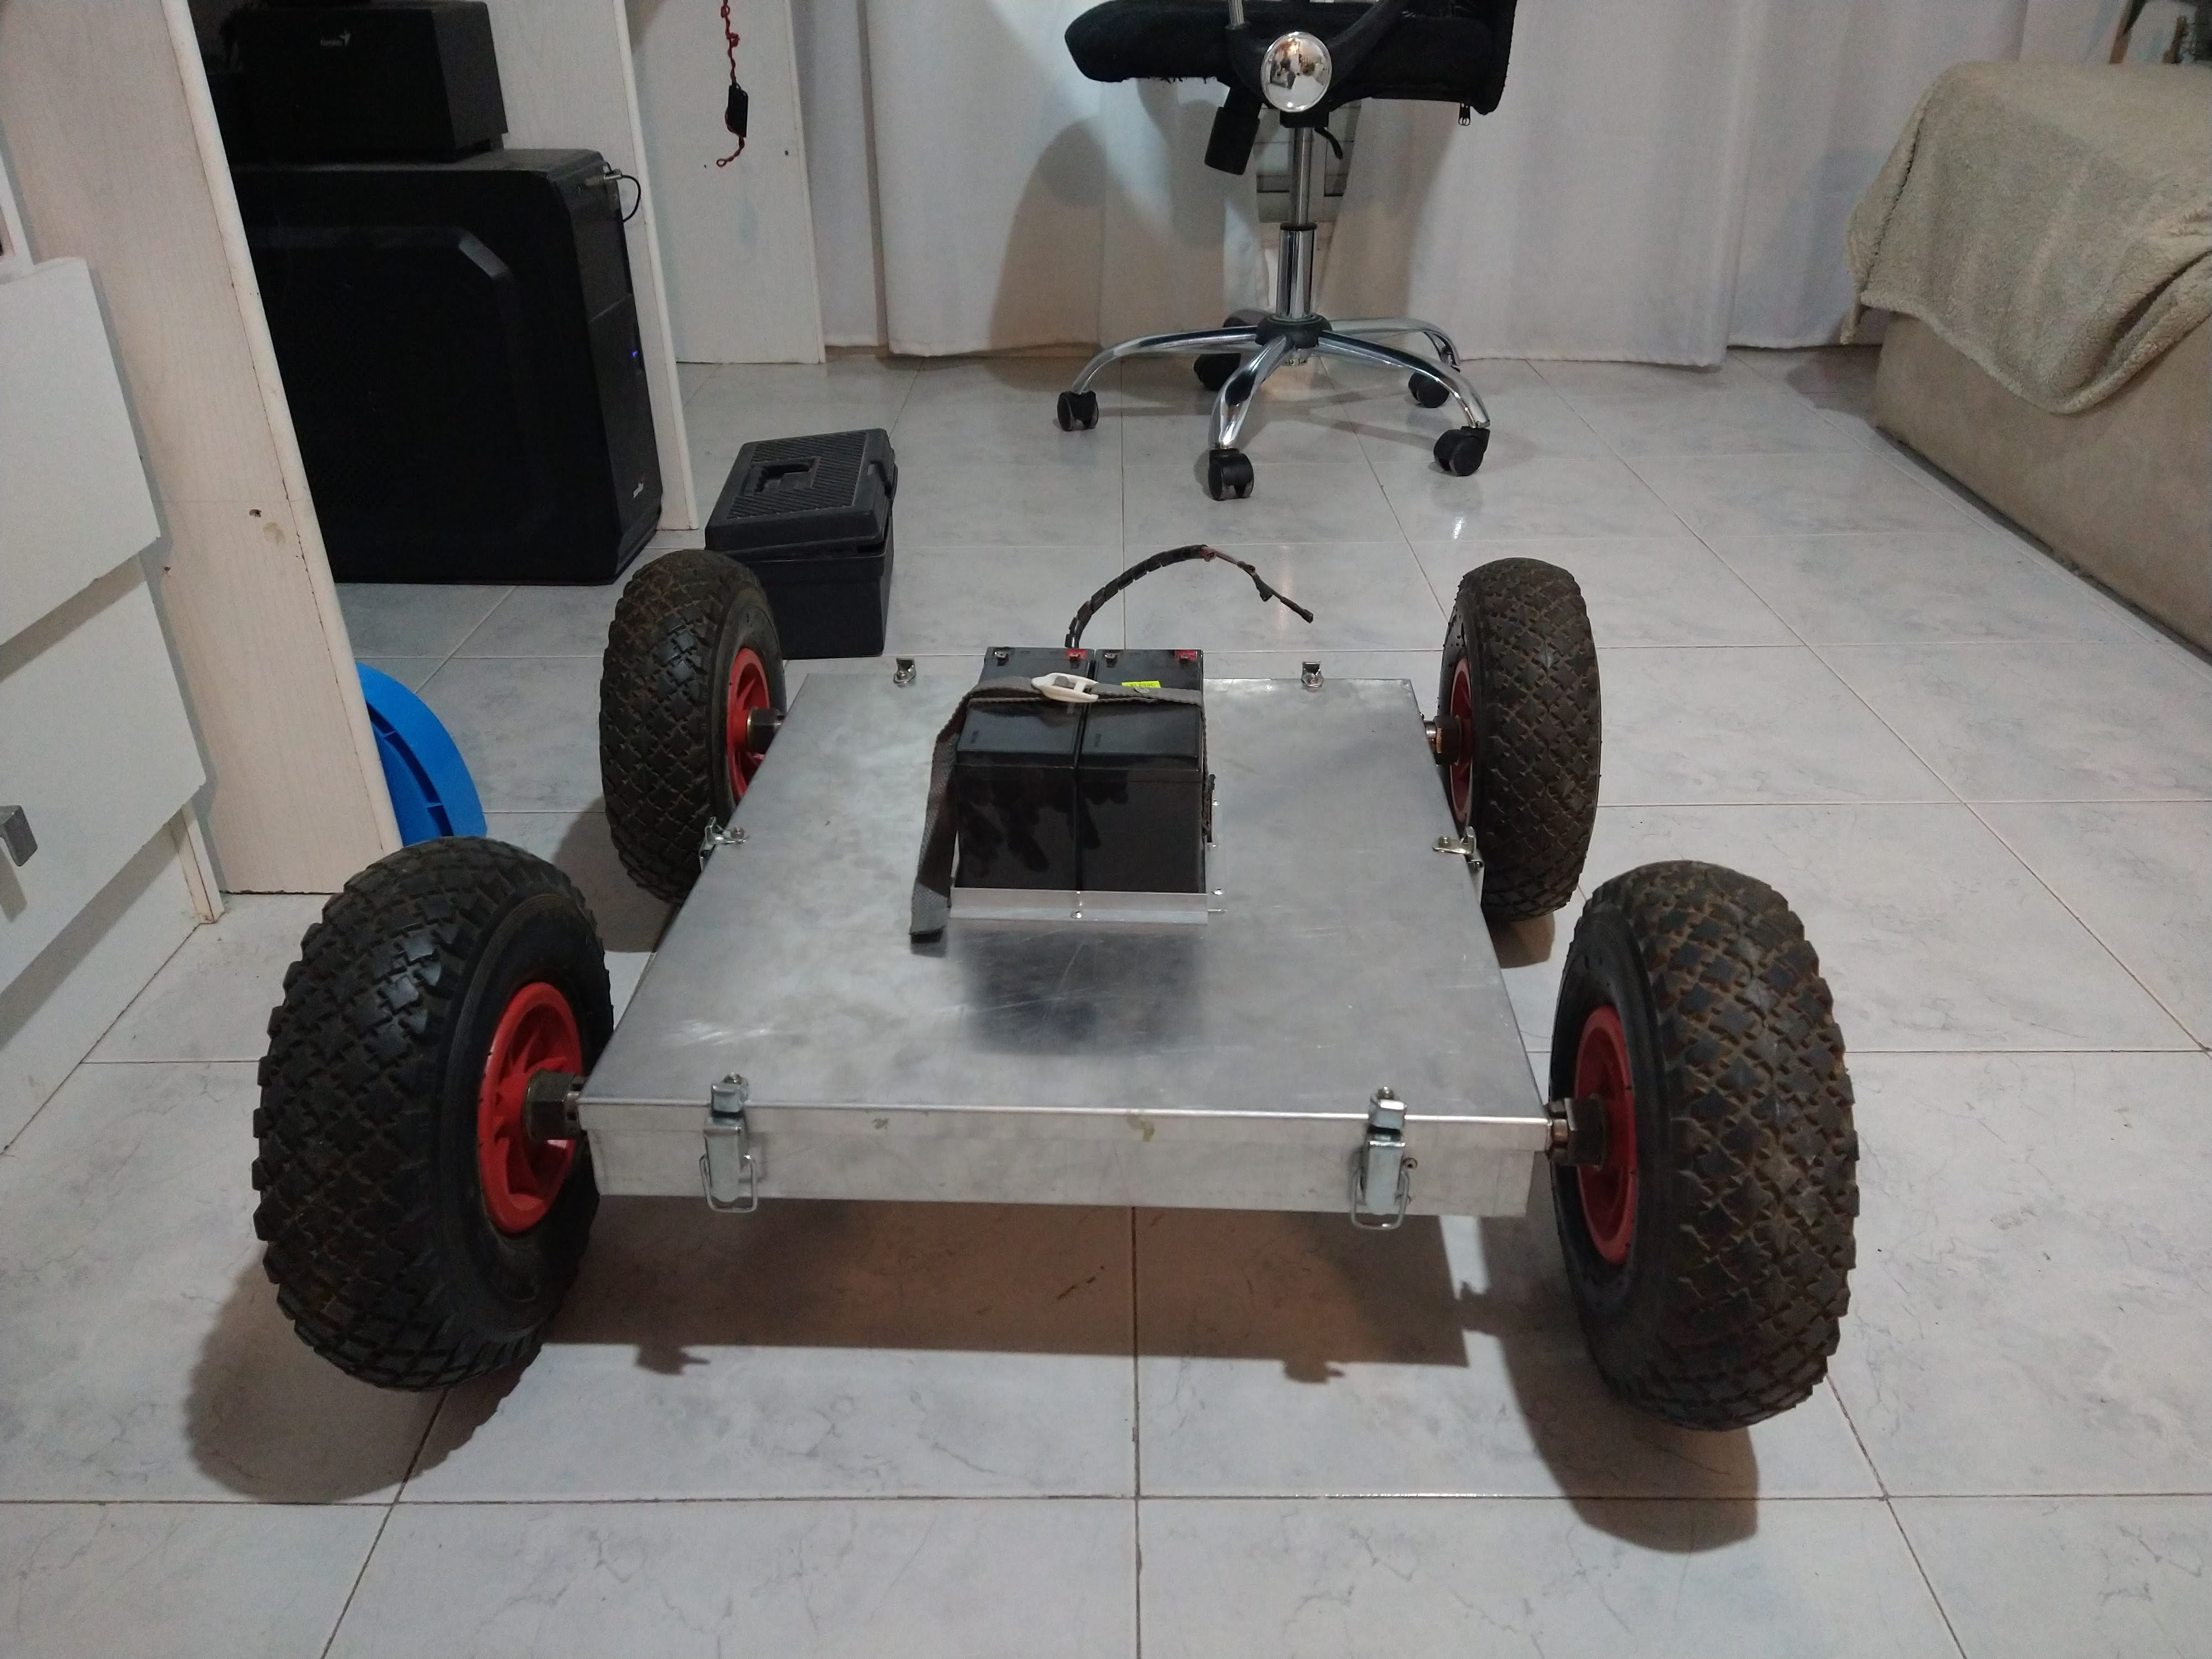
\includegraphics[scale = 0.1]{img/FotoDePresentacion.jpg}

